\section*{Supplementary Information}
\phantomsection
\addcontentsline{toc}{section}{Supplementary Information}

\renewcommand{\thefigure}{S\arabic{figure}}
\setcounter{figure}{0}

\begin{figure}[ht]
    \centering
    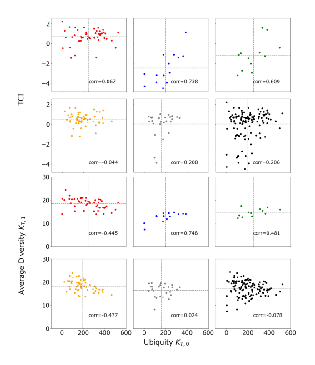
\includegraphics[scale=2.75]{Figs/FigA1.eps}
    \caption{The Pearson correlation between the degree centrality \( K_{T,0} \) of technology node \( T \) classified by IPC and the average nearest neighbor degree \( K_{T,1} \), and the Pearson correlation between the degree centrality \( K_{T,0} \) of technology field node \( T \) and TCI. In both figures, the black lines indicate the mean values. Each data point is color-coded according to the five classifications defined by Schmoch\cite{Schmoch2008}.}
    \label{fig:persector}
\end{figure}

\begin{figure}[ht]
    \centering
    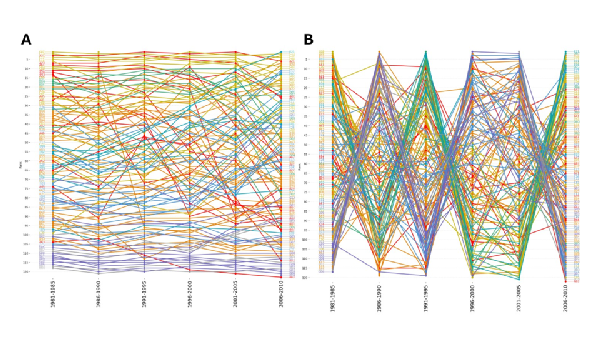
\includegraphics[scale=1.75]{Figs/FigA2.eps}
    \caption{Changes in the five-year rolling ranking of the TCI based on 124 three-digit IPC classes for
      (A) the corporate analysis and
      (B) the regional analysis.
      The lines color-coded according to the one-digit IPC classes.
    }
    \label{fig:bump}
\end{figure}

\begin{figure}[ht]
    \centering
    
\includegraphics[scale=0.75]{Figs/FigA3.eps}
    \caption{The distribution of weighted patent counts (horizontal axis) for each corporation, with the cumulative distribution function (CDF) of their patents on the vertical axis. The black dashed lines on both axes indicate the excluded region, corresponding to the top 3\% of corporations that account for 93\% of all patents.}
    \label{fig:patentdistribution}
\end{figure}

